\chapter{Linked List}
\label{chap:linked-list}

\section{Introduction}
\label{sec:introduction-linked-list}


\section{Types of Linked List}
\label{sec:types-of-linked-list}

\begin{figure}[H]
  \centering
  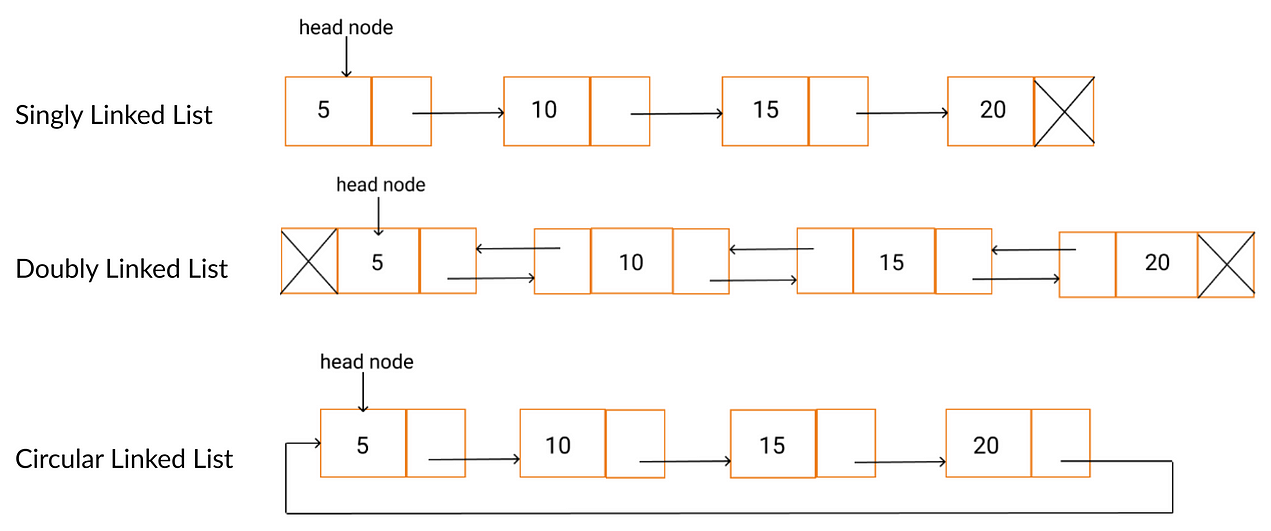
\includegraphics[width=0.8\textwidth]{Figures/pimg10.png}
  \caption{Different Types of Linked List}
  \label{fig:pimg10--singly-linked-list-visualization}
\end{figure}

\section{Singly Linked List}
\label{sec:singly-linked-list}

\begin{figure}[H]
  \centering
  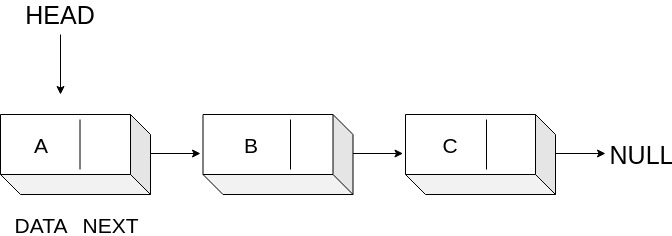
\includegraphics[width=0.8\textwidth]{Figures/pimg7.png}
  \caption{Singly Linked List Visualization}
  \label{fig:pimg7--singly-linked-list-visualization}
\end{figure}

\subsection{Implementation of Singly Linked List}
\label{ssec:implementation-of-singly-linked-list}

\begingroup
\label{lst:deque-implementation}
\inputminted[breaklines]{python}{Code/singly_linked_listwith_tail.py}
\captionof{listing}{Singly Linked List with Tail Implementation}
\endgroup

\section{Doubly Linked List}
\label{sec:doubly-linked-list}

\begin{figure}[H]
  \centering
  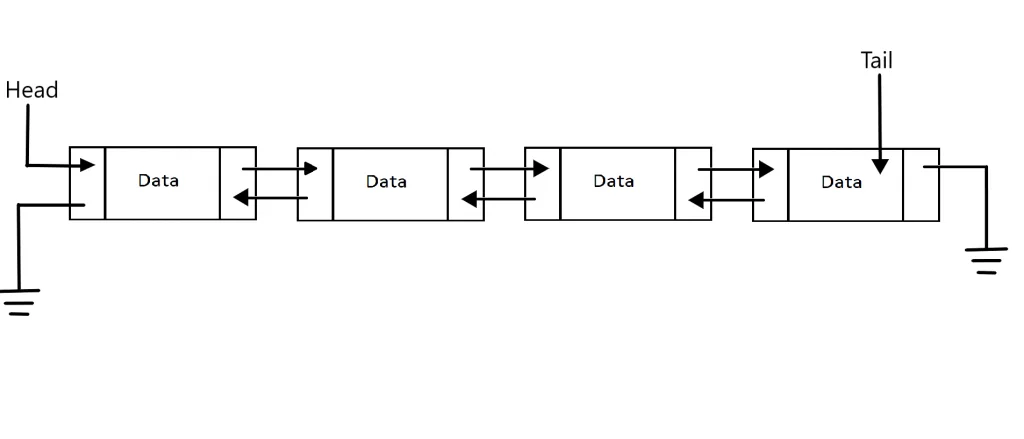
\includegraphics[width=0.8\textwidth]{Figures/pimg9.png}
  \caption{Doubly Linked List Visualization}
  \label{fig:pimg9--cicular-linked-list-visualization}
\end{figure}

\subsection{Implementation of Doubly Linked List}
\label{ssec:implementation-of-doubly-linked-list}

\begingroup
\label{lst:deque-implementation}
\inputminted[breaklines]{python}{Code/doubly_linked_list.py}
\captionof{listing}{Doubly Linked List with Tail Implementation}
\endgroup

\section{Circular Linked List}
\label{sec:circular-linked-list}

\begin{figure}[H]
  \centering
  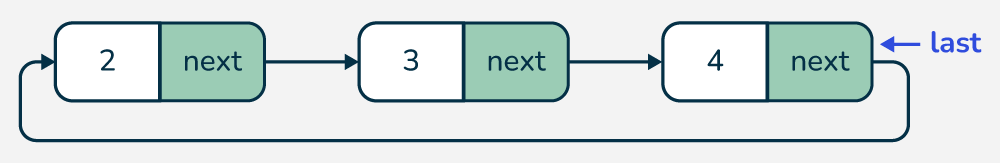
\includegraphics[width=0.8\textwidth]{Figures/pimg8.png}
  \caption{Circular Linked List Visualization}
  \label{fig:pimg8--cicular-linked-list-visualization}
\end{figure}
